\section{Experimental Evaluation}
\label{sec:experiments}

Our experimental evaluation aims to answer the following questions: (1)~Does \Acronym{} enable VLAs to perform tasks that require long-term memory spanning up to 15~minutes? (2)~Does \Acronym{} unlock new capabilities in VLA models, like in-context adaptation of manipulation strategies, based on short-term memory of recent failures? (3)~How does the performance of \Acronym{} compare to prior approaches for adding memory to VLA models?




\subsection{\Acronym{} Solves Tasks Requiring Long-Horizon Memory}
\label{sec:challenge_tasks}

\begin{figure*}
    \centering
    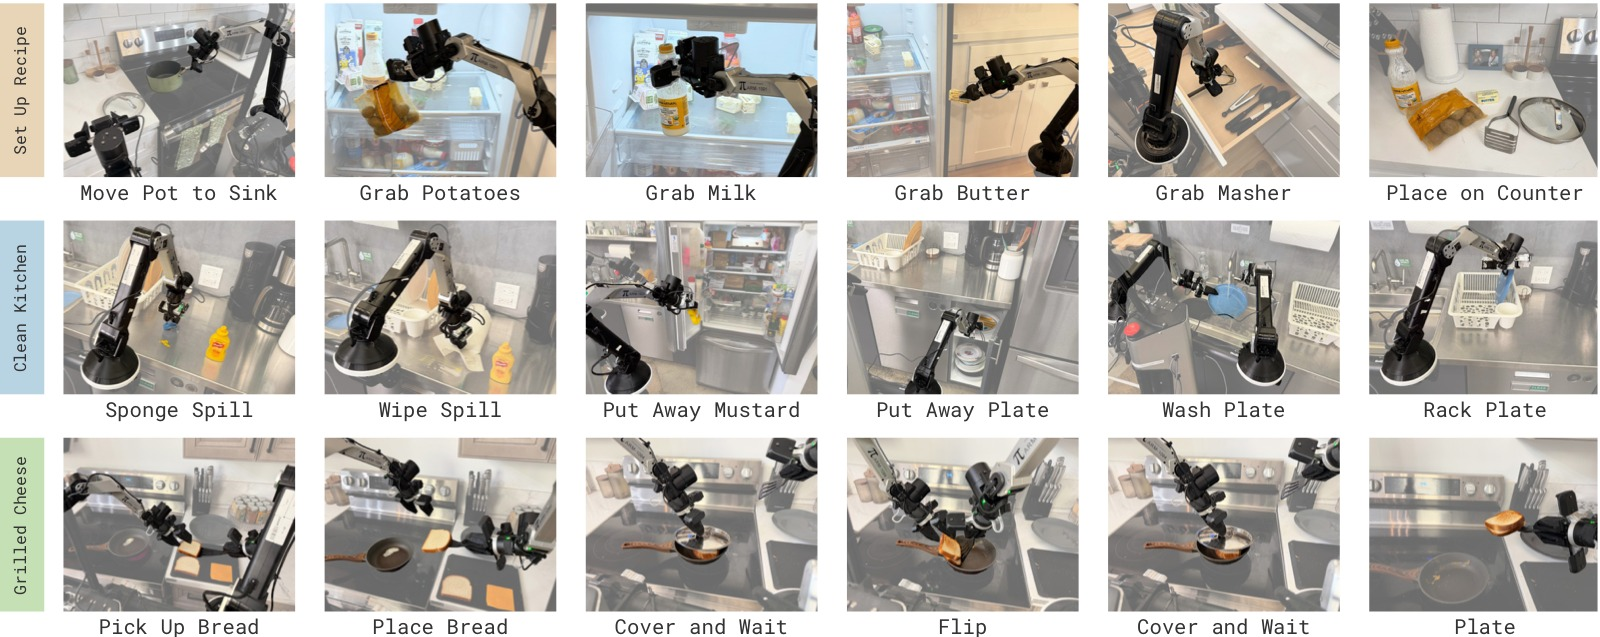
\includegraphics[width=\textwidth]{figures/long_horizon_no_highlight.pdf}
    \caption{\small{We test \Acronym{} policies across multiple challenging, long-horizon dexterous manipulation tasks that require retaining memory for up to fifteen minutes, including setting up a recipe, cleaning up a kitchen (\cref{sec:challenge_tasks}), and making a grilled cheese sandwich (\cref{sec:analysis}).}}%
    \label{fig:challenge_tasks}
\end{figure*}

We evaluate our method's potential for enabling long-horizon tasks using two challenging scenarios that require retaining memory for up to fifteen minutes (see \cref{fig:challenge_tasks}, rows 1 \& 2): (1)~\textbf{Recipe setup}: The robot is given a detailed prompt specifying the ingredients and cookware required to cook a recipe and their location, and is asked to fetch all of them from various cabinets, drawers, or, e.g., the fridge, and place them at a specific location, e.g., on the stove or a specific countertop. Memory is required to keep track of all items that have already been assembled and remember to close drawers, cabinets, or the fridge once the task is complete. We train on 42~recipes across diverse kitchen scenes, and evaluate on five of the recipes in unseen kitchens and with unseen objects.
(2)~\textbf{Clean up kitchen}: The robot needs to clean up a messy kitchen environment, including stowing objects in the fridge, wiping countertops, washing dishes with soap and running water, and placing dishes in the drying rack. Memory is required for remembering steps in the cleanup process (e.g., whether soap has been added to the dishes before washing, whether both front and back of the dish have been washed), remembering which surfaces have already been cleaned, and remembering to close cabinets after objects have been stowed. This task is not only challenging from a memory perspective, but also requires policies to perform multiple dexterous manipulations, from wiping surfaces to carefully handling water and soap. For more details on training data, evaluation conditions, and scoring rubrics for progress scores, see \cref{sec:task_details}. All evaluations use \nchallengerollouts{}~rollouts per policy and task or recipe, and we report mean $\pm$ standard error in all graphs.

\begin{figure}
    \centering
    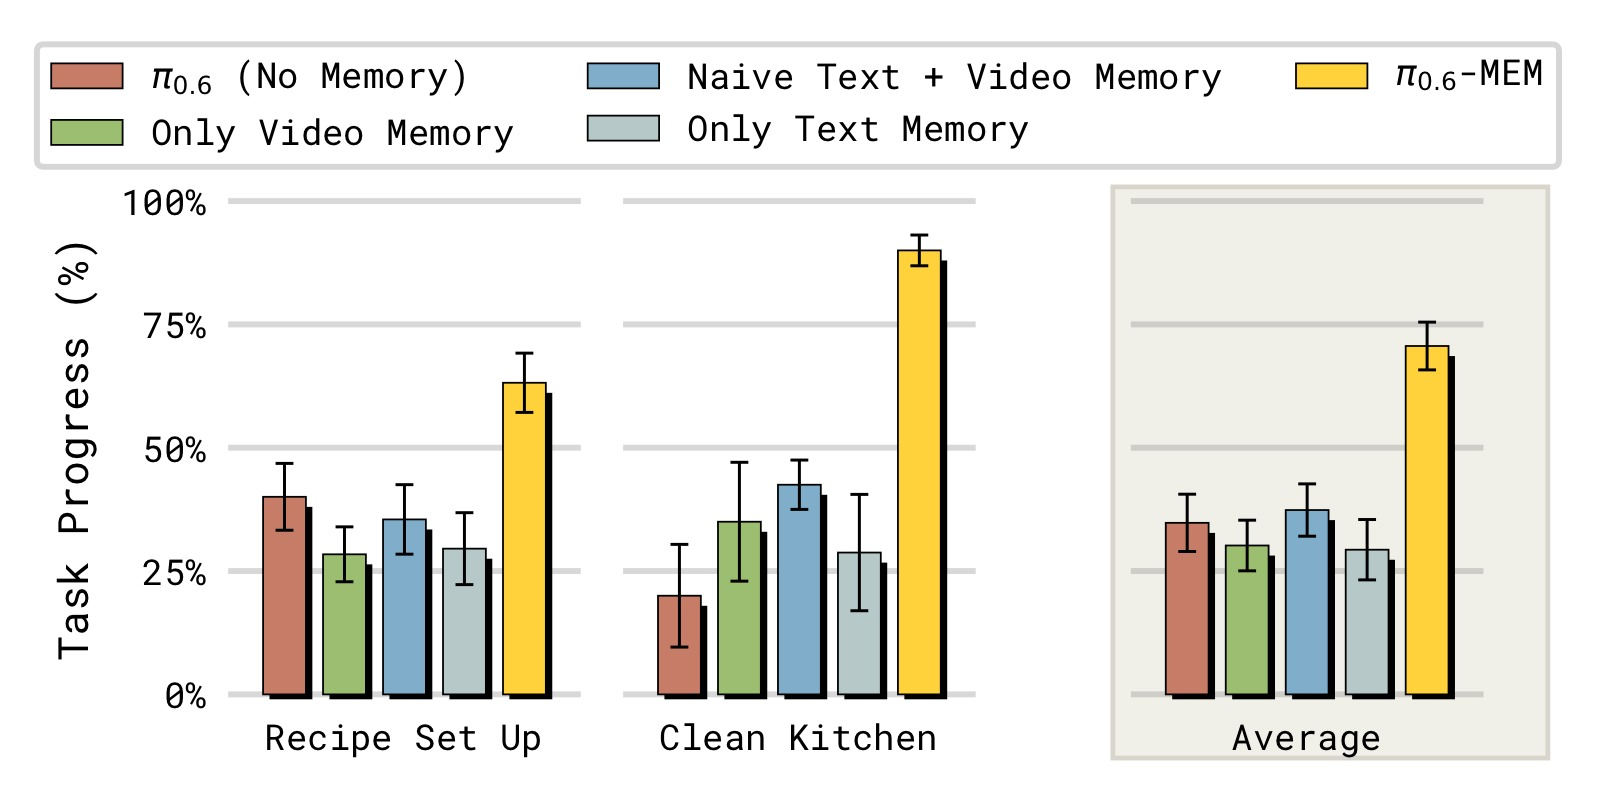
\includegraphics[width=\linewidth]{figures/flagship_tasks_bottom.pdf}
    \caption{\small{Performance of policies on challenging, long-horizon manipulation tasks. Without memory, even state-of-the-art generalist policies like \pizerosix{} struggle to perform such tasks. We ablate the memory components and show these tasks are solvable by combining short-horizon, observation-based memory, with long-horizon, language-based memory. Naive memory of past language instructions, without compression, struggles with training-inference distribution shifts.}}
    \label{fig:challenge_tasks_results}
\end{figure}


\cref{fig:challenge_tasks_results} shows the results: without memory, even state-of-the-art models like \pizerosix{} struggle to perform these challenging long-horizon tasks. While prior works have shown policies that perform manipulation over extended periods of time~\citep{intelligence2025pi}, 
solving real-world tasks with flexible subtask sequences and frequent partial observability fundamentally requires memory. %
The results show that \Acronym{} is effective at providing the required context to the policy across both short and long-horizon time intervals, and increases policy success rate significantly.

To better understand what contributes to \pizerosix{}-\Acronym{}'s strong performance, we perform a detailed ablation study of the different components of our approach. We report the results in \cref{fig:challenge_tasks_results}. We compare to versions of our policy that \emph{remove} short-horizon video memory or long-horizon language memory, and show that both are essential to solving the challenge tasks. Without video memory, the robot may struggle to understand how long it has been washing a plate or wiping a surface, and get ``stuck'' indefinitely. Video memory also helps robustify manipulation tasks via in-context adaptation (see \cref{sec:in_context_exp}). Long-horizon language memory, on the other hand, is essential for remembering semantic events in the more distant past. It allows the policy to keep track of steps in the recipe, or remember to close doors that it has opened. We also evaluate a version of our policy that removes the \emph{compression} applied to the language-based memory (see \cref{sec:language_memory}): instead of training the model to compress and discard information that is no longer needed, we simply concatenate all previous subtask instructions up to a maximum length in the input of the high-level policy. We find that this type of ``naive'' language memory works significantly worse than our model-predicted summaries. The core challenge with ``naive'' language memory is a large train-inference distribution shift: during training, most episodes utter any given subtask instruction only once (e.g., ``\texttt{pick up bowl}'' $\rightarrow$ ``\texttt{place bowl in cabinet}'') since they are typically near-optimal human demonstrations. Yet, during inference time policies may repeatedly fail on a given subtask, causing the high-level policy to repeatedly produce the same subtask before finally succeeding and moving on (``\texttt{pick up bowl}'' $\rightarrow$ ``\texttt{pick up bowl}'' $\rightarrow$ ``\texttt{pick up bowl}'' $\rightarrow$ ``\texttt{place bowl in cabinet}''), leading to a distribution shift that can degrade overall policy performance. In contrast, \Acronym{}'s language memory mechanism would simply not update the memory representation until the bowl was successfully picked up. This \emph{compression} of context (e.g., discarding failed attempts) thus reduces distribution shift and improves overall performance. 

\subsection{In-Context Adaptation of Manipulation Strategies}
\label{sec:in_context_exp}

\begin{figure}
    \centering
    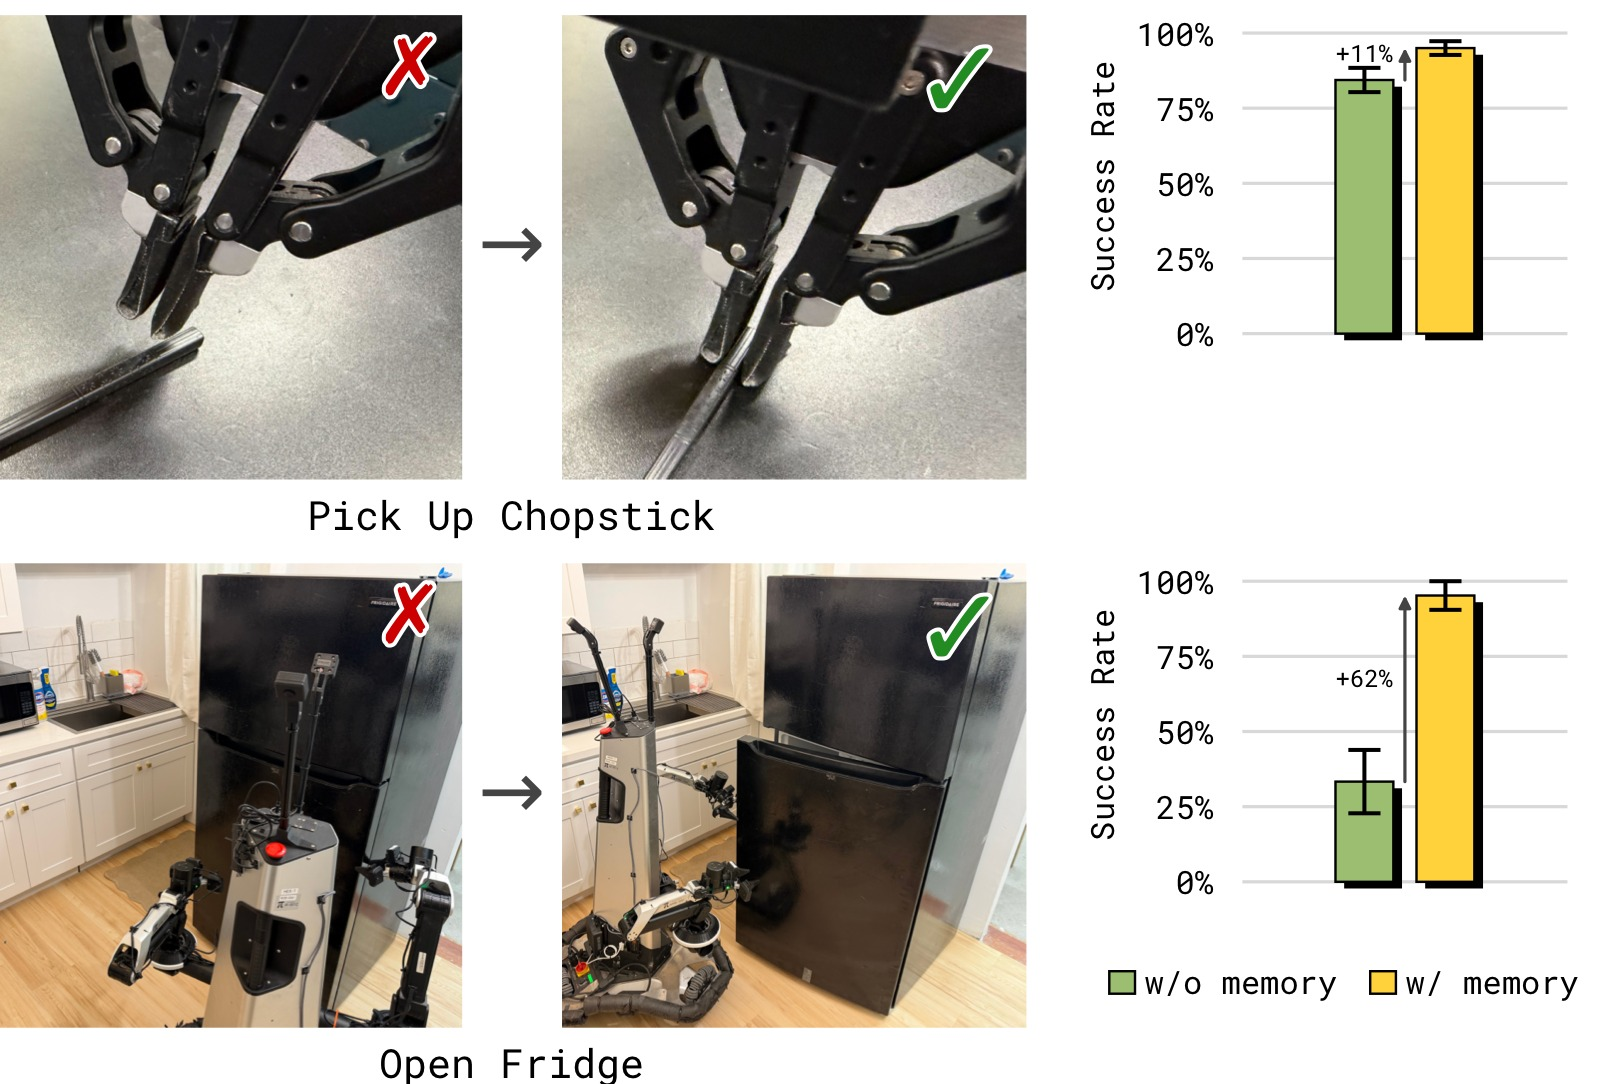
\includegraphics[width=\linewidth]{figures/in_context_pct.pdf}
    \caption{\small{VLAs with memory can perform in-context adaptation of manipulation strategies, like adjusting grasp height or door opening direction. Without memory, policies get stuck with a suboptimal strategy.}}
    \label{fig:in_context_adapt}
\end{figure}

In the previous section, we showed that \Acronym{} can enable VLAs to solve very long-horizon tasks. In this section, we investigate whether equipping VLAs with memory can unlock improved performance, even on shorter-horizon tasks that at first glance may not require memory. Intuitively, while memory across tens of minutes is useful for keeping track of overall task progress, short-horizon memory can enable policies to \emph{adapt} their behavior \emph{in-context} and intelligently react to mistakes: instead of failing in the same way over and over, policies can use context of previous failed attempts to, for example, modify the way in which they are trying to pick up an object, or how they open a door. 

To test whether \Acronym{} unlocks such in-context adaptation, we set up two tasks on which current state-of-the-art VLAs like \pizerosix{} struggle (\cref{fig:in_context_adapt}): picking up flat objects like chopsticks with an out-of-distribution table height, which leads to frequent mis-grasps, and opening fridges where the direction the door opens is unclear, resulting in repeated failed opening attempts.


To teach policies the in-context adaptation strategy, we follow~\citep{intelligence2025pi} and collect targeted human feedback: after the policy fails, a human intervenes and provides a demonstration of the corrected manipulation strategy, like adjusting grasp height for picking up the chopstick. For the fridge-opening task, we collect exploration rollouts in which the demonstrator initially does not know the opening mechanism, so the data naturally contains both the failed attempt and the subsequent corrective demonstration. We then simply finetune the \pizerosix{}-\Acronym{} policy with this correction data, keeping the failed attempt that preceded the correction in the short-term memory of the model during training. As a result, the model learns to adapt its manipulation strategy when it sees a mistake in its short-term memory. We compare to finetuning the memoryless \pizerosix{} policy on the same intervention data.



The results in \cref{fig:in_context_adapt} show that the \Acronym{}-VLA with memory is much more effective at leveraging the corrections, and learns to adapt its manipulation strategy on the fly. The policy without memory has no way to remember which strategy was attempted before, and therefore cannot intelligently change the strategy after a mistake.
In contrast, policies with memory can use the context to understand which strategy has already been tried and failed, and adjust accordingly.



\subsection{Analysis Experiments}
\label{sec:analysis}

\begin{figure*}[t]
    \centering
    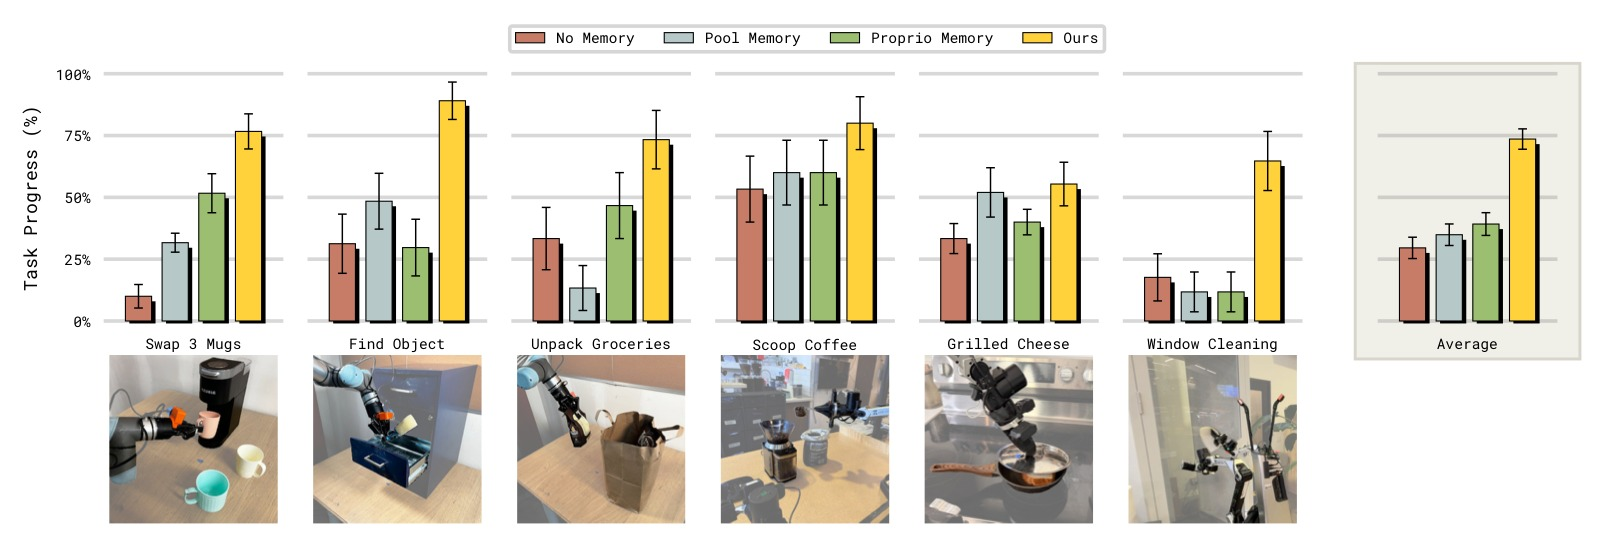
\includegraphics[width=\textwidth]{figures/history_ablation_bottom.pdf}
    \caption{\small{Comparison of approaches for equipping VLAs with memory across core memory capabilities (handling partial observability, counting, visual memory). VLAs without memory struggle to perform these tasks. Only \Acronym{}'s memory approach performs well across all core capabilities.}}
    \label{fig:analysis_results}
\end{figure*}

\textbf{Tasks.} To compare our method to existing approaches that equip VLAs with memory across a wide range of capabilities, we develop a suite of challenging manipulation tasks that measure the ability of policies to use memory efficiently, and perform dexterous manipulations (see \cref{fig:analysis_results,fig:dexterous_results} for task visualizations). %
The tasks span a diverse set of scenarios involving single-arm, dual-arm, and mobile robots. They test for core memory capabilities, like handling \textbf{partial observability} (e.g., remembering which drawer an object was placed in by a human; unpacking a grocery bag and remembering whether objects are left to unpack; placing and removing multiple mugs under a coffee machine), \textbf{counting} (e.g., counting scoops of coffee to add to a coffee grinder), timing (e.g., remembering how long a grilled cheese sandwich has been cooking, see \cref{fig:challenge_tasks}), and \textbf{spatial memory} (e.g., remembering which parts of a window have already been wiped). They also require policies to perform \textbf{precise manipulations} (e.g., folding a stack of laundry or assembling a cardboard box). They are thus well-suited to test the limits of existing memory approaches and also compare to the performance of state-of-the-art VLAs without memory. Following prior work~\citep{blackpi0}, we collect small post-training datasets for the most challenging manipulation tasks and for the memory tasks, and evaluate policies out-of-the-box for all remaining tasks (\cref{fig:dexterous_results}).
We provide detailed descriptions of all task setups in \cref{sec:task_details}.





\textbf{Comparisons.} A number of prior works leverage observation-based (shorter-horizon) memory, and address its computational challenges through aggressive compression of observations from past timesteps. We compare our approach to two representative prior works to understand the tradeoffs of different memory representations: (1)~\textbf{Pool Memory} akin to \citet{jang2025contextvla}, we
compress all past observations into a single ``memory token'' using average pooling. We implement it by encoding each of the past observations separately with the pre-trained single-frame ViT, and then applying an average pooling operation on the frame encodings before passing them into the VLA backbone. The current timestep's observation is separately encoded and passed into the VLA without pooling; (2)~\textbf{Proprio Memory} conditions on a history of low-dimensional robot states only, akin to~\citep{zhang2025ta}, to avoid the computational cost of high-dimensional image memory. All proprioceptive states from past timesteps are separately passed through a linear projection, and then fed into the VLA backbone. To ensure fair comparison, we re-implement all approaches on top of the \pizerosix{} VLA backbone and use a version of our model \emph{without} language-based long-horizon memory. To test the performance of our policy on the most dexterous tasks, we also compare to \textbf{\pizerosix{}} \emph{without} memory, a state-of-the-art VLA that has shown strong results on complex manipulation tasks~\citep{pi06_model_card}. Finally, to better understand the effect of \emph{pre-training} on memory efficacy, we compare to \textbf{\Acronym{}-Posttrain-Only}, an ablation of our method that introduces the video encoder only during \emph{post-training} on the target task, starting from the pre-trained \pizerosix{} checkpoint, akin to \citet{li2025cronusvla}.



We report results in \cref{fig:analysis_results}. We first compare the different memory approaches on tasks that test core memory capabilities (\cref{fig:analysis_results}). As expected, the \pizerosix{} VLA \emph{without} memory struggles on these tasks and often has to resort to random chance, e.g., when picking which of four drawers to open to find the object hidden inside (25\% success) or whether or not to add another scoop of coffee (50\% success). In contrast, existing memory solutions improve performance, particularly on simpler memory tasks that only require a few bits of memory, e.g., remembering how many scoops of coffee have already been added to the hopper. We find that Pool-Memory's aggressive observation compression via average-pooling can lead it to struggle particularly on tasks that require longer-term memory, like remembering the past positions of multiple coffee mugs or recalling how many objects are left to unpack in a grocery bag. Proprio-Memory on the other hand is only effective in tasks where the robot needs to remember \emph{its own} state, but struggles in scenarios where remembering the \emph{environment} state is necessary: e.g., recalling which drawer contains a particular object.

\begin{figure}
    \centering
    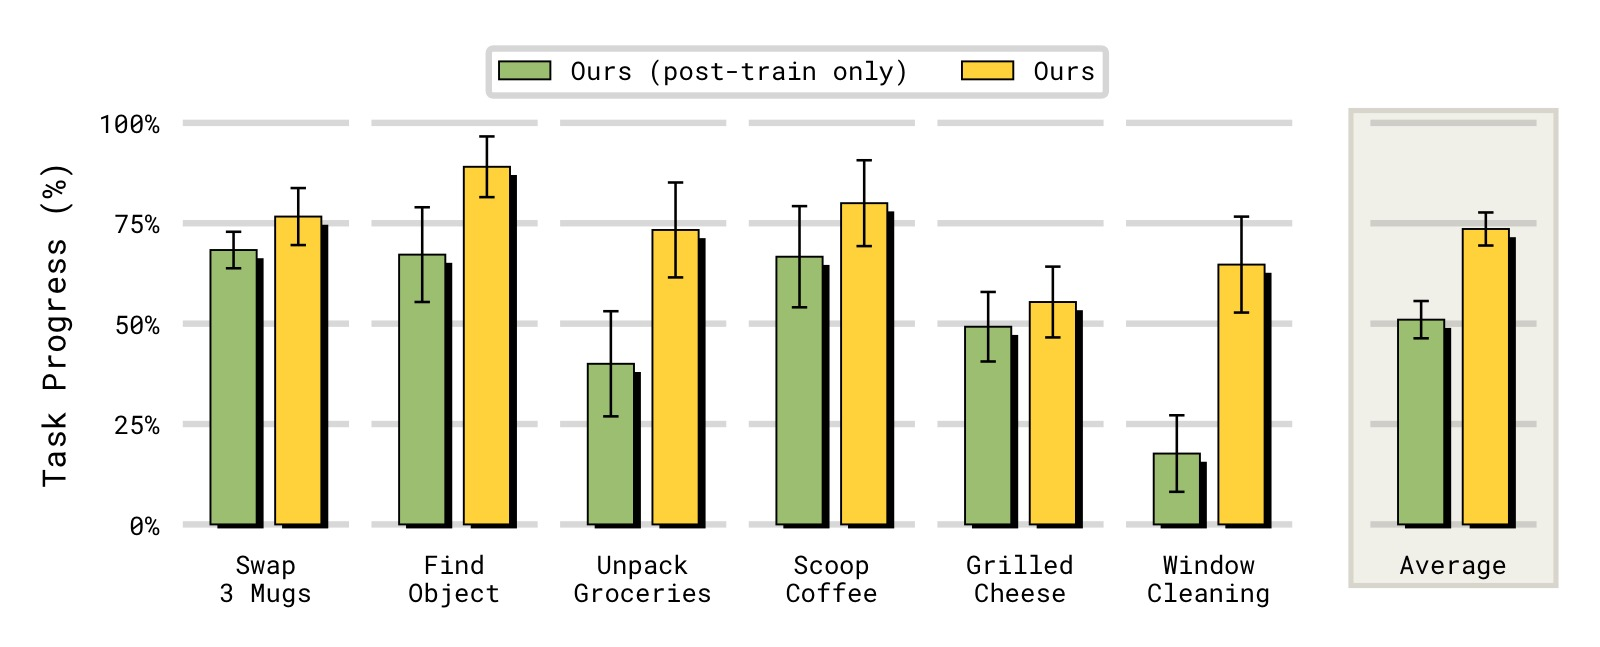
\includegraphics[width=\linewidth]{figures/posttrain_ablation_bottom.pdf}
    \caption{\small{Pre-training \Acronym{} on a diverse dataset of robot and non-robot video data makes it more effective at using its memory to solve diverse manipulation tasks. Introducing memory during post-training only results in substantially lower performance.}}
    \label{fig:posttrain_ablation}
\end{figure}

In comparison, the \Acronym{} VLA is the only model that achieves strong performance across \emph{all} tested memory capabilities. It can reliably handle partial observability challenges like remembering the location of objects, and also leverage these capabilities in dexterous tasks like unpacking a bag of groceries. Notably, pre-training the observation-based memory on a diverse data mix of robot and non-robot data significantly improves the ability of the model to leverage its memory -- even when the memory horizon is significantly expanded during post-training (e.g., from 5~seconds in pre-training to up to 1~minute in post-training). The version of our model that only introduces memory during post-training is noticeably worse at leveraging the information from past timesteps (see \cref{fig:posttrain_ablation}). We emphasize that this model is still initialized from a base \pizerosix{} checkpoint pre-trained on the same diverse robot data, but did not develop memory capabilities during this pre-training. Finally, the head-to-head comparison of Ours (post-train only) vs. Pool-Memory demonstrates that even without pre-training, our video encoder design is a more effective approach for extracting information from prior timesteps than separately encoding each timestep and average pooling. By interleaving temporal attention operations throughout the layers of the ViT, our video encoder can more effectively extract and compress the relevant information.


\begin{figure*}[t]
    \centering
        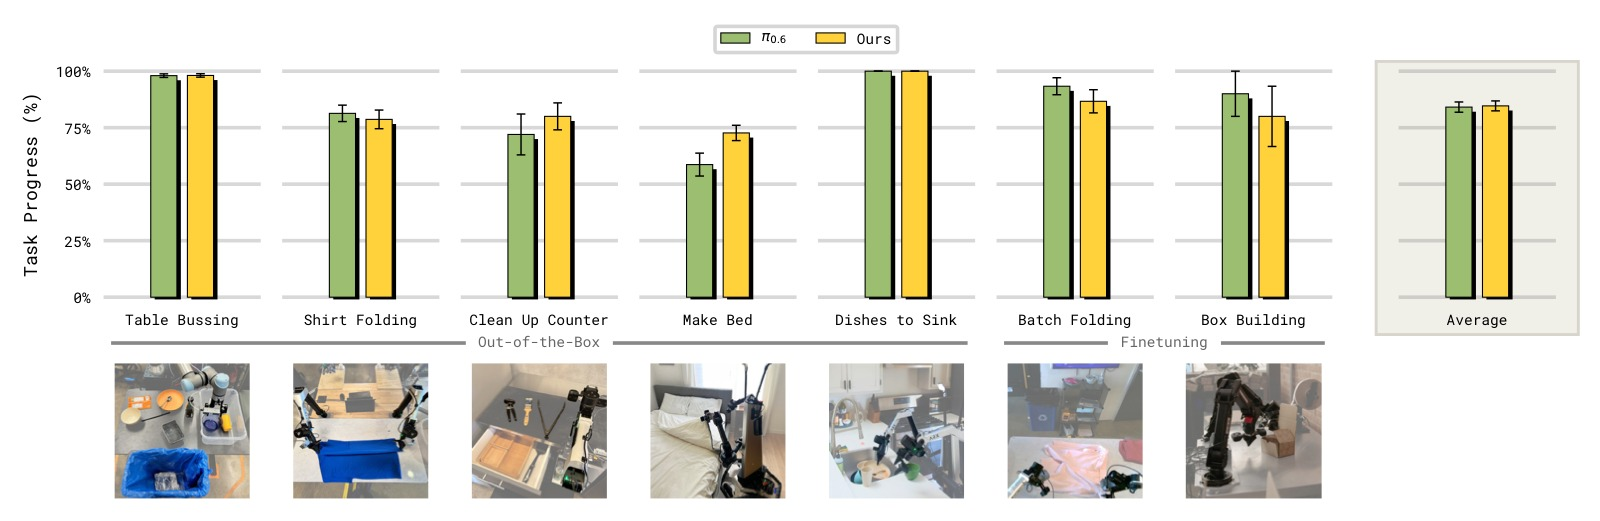
\includegraphics[width=\textwidth]{figures/nohistory_ablations_bottom.pdf}
    \caption{\small{In addition to effectively using its memory, \Acronym{} also matches the performance of state-of-the-art non-memory VLAs across challenging manipulation tasks that do not require memory.}}
    \label{fig:dexterous_results}
\end{figure*}

In addition to testing core memory capabilities, we also test the performance of \Acronym{} across a range of challenging dexterous manipulation tasks (\cref{fig:dexterous_results}). We find that the \Acronym{} VLA not only makes effective use of memory in tasks that require it, but it can \emph{also} match the state-of-the-art performance of the \pizerosix{} VLA across challenging dexterous manipulation tasks. This is notable, since numerous previous works have reported degradations in performance from adding memory to policies, e.g., due to causal confusion~\citep{chi2025diffusion, zheng2024tracevla}. We attribute \Acronym{}'s strong performance in large parts to our diverse pre-training data mixture, which contains episodes of varying optimality, speed, and control frequency, in addition to diverse internet videos. Together, this diversity can prevent spurious correlations in the video encoder that may arise when training on smaller, more uniform robot datasets, and lead to the brittleness and performance degradation of policies with memory reported in prior work. %






















